%!TEX root = ../physical-olympics-2.tex
\chapter{光的干涉}


\section{标量波理论}
标量波是指以下标量偏微分\emph{波动方程}(wave equation)的解:
\[\left(\nabla^2 -\frac{1}{c^2}\frac{\partial^2}{\partial t^2}\right)A(\bs{r},\,t)=0\]

分别在直角坐标,\,柱坐标,\,球极坐标下用所谓的分离变量法可以得到一些正确的基础解\footnote{以下三式都要求$\omega >0$,\,数学上看$\omega<0$也没错,\,但是利用三角函数的性质可以将$t$系数变号而不带来新的解.}:
\begin{figure}[H]
\centering
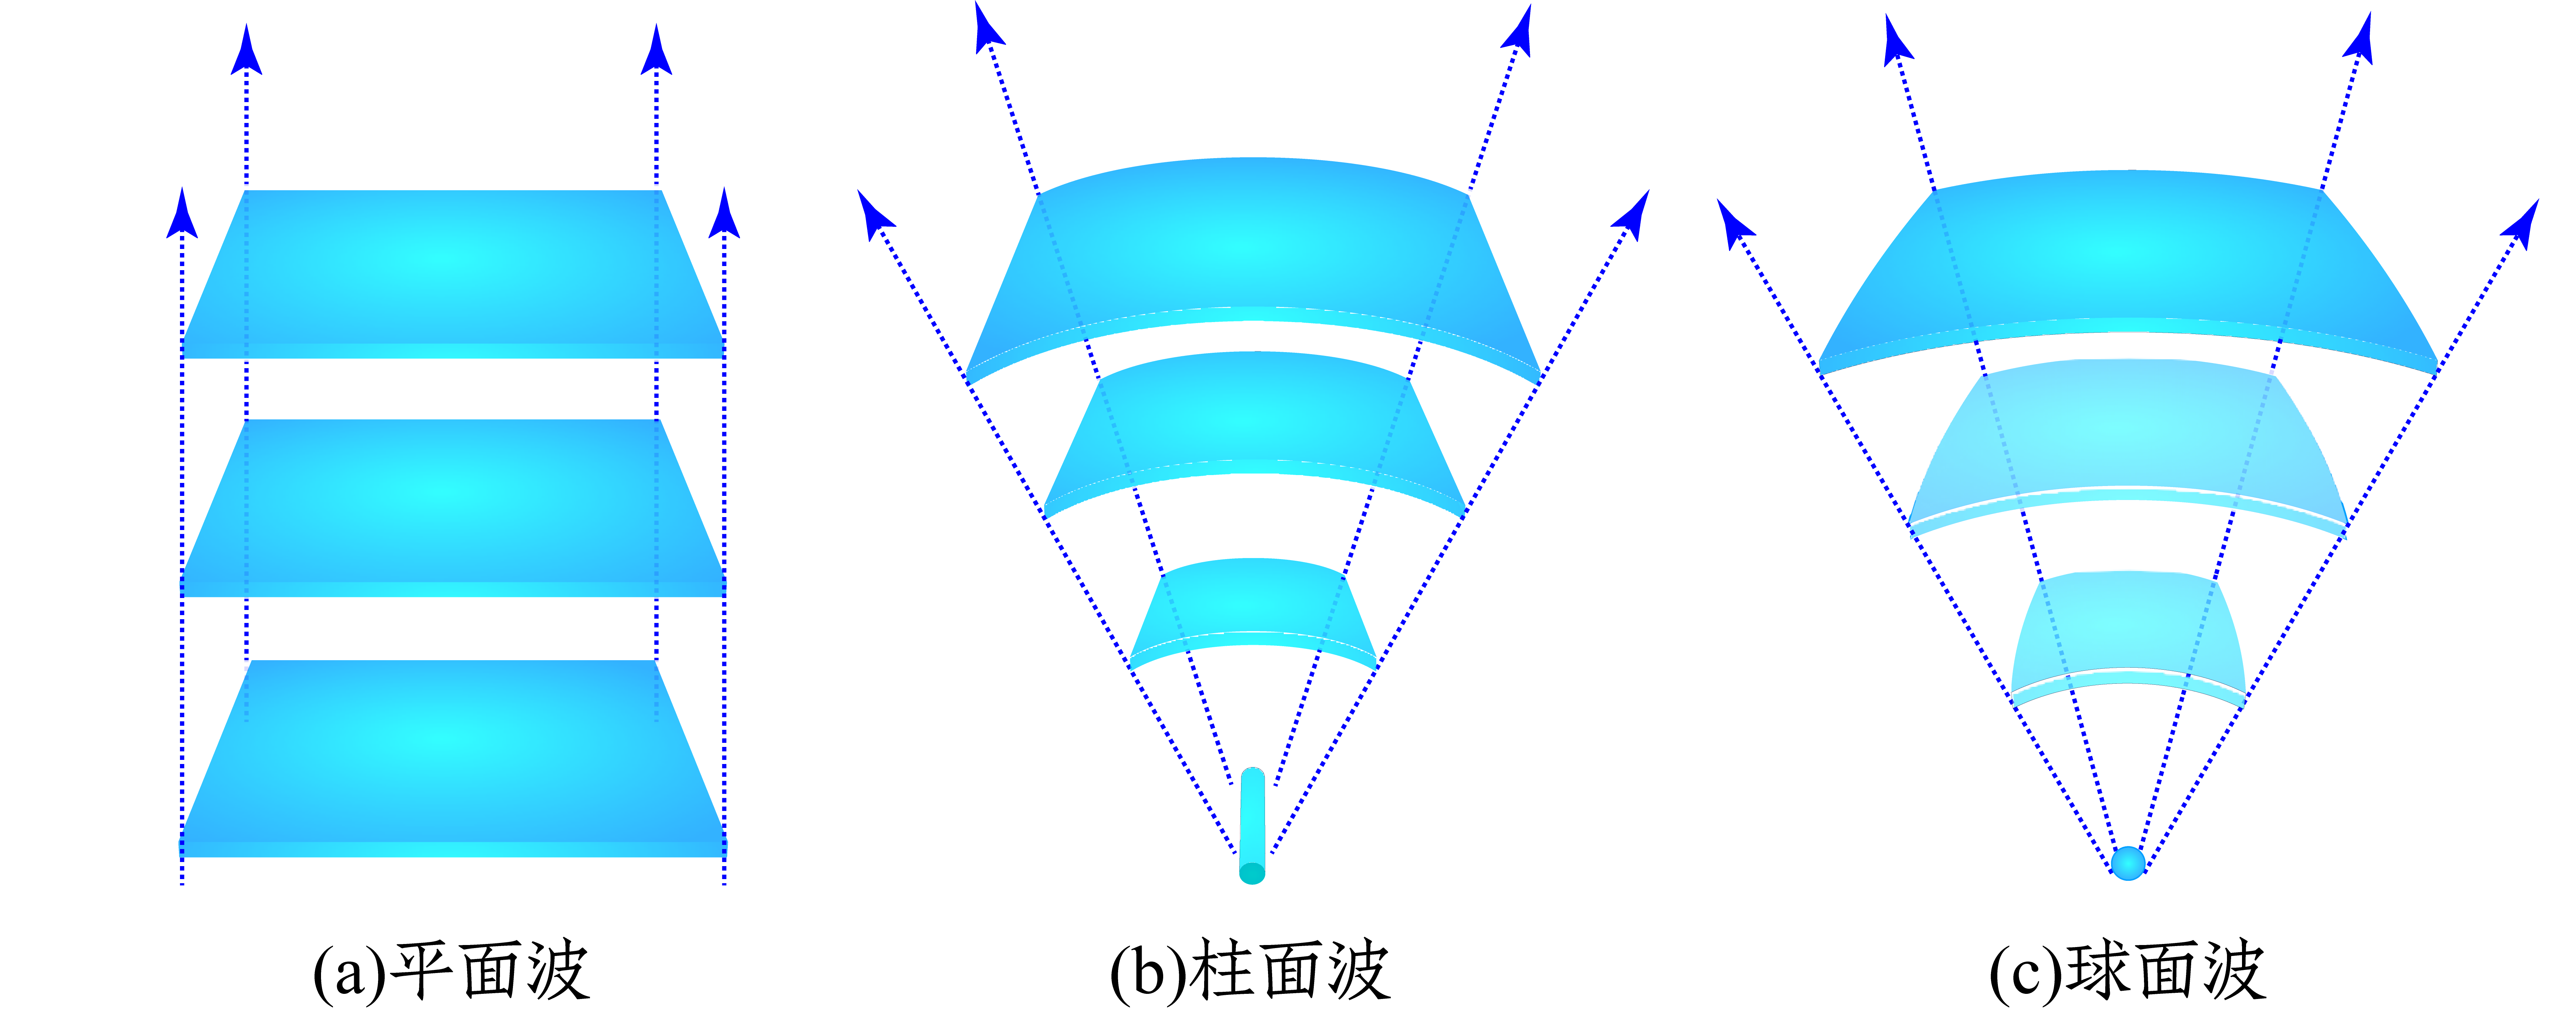
\includegraphics[width=0.8\textwidth]{image/14-1-1.png}
\caption{三种典型的波}
\end{figure}

\begin{enumerate}
	\item $A(\bs{r},\,t)=A\cos(\omega t-\bs{k}\cdot \bs{r}+\phi)$

	要求$\dfrac{\omega}{|\bs{k}|}=c$.\,此为传播方向为$\bs{k}$的平面行波.
	\item $A(\bs{r},\,t)=\dfrac{I}{\sqrt{\rho}}\cos(\omega t-k\rho+\phi)$

	要求$\dfrac{\omega}{|k|}=c$.\,$k>0$时为向外传播的柱面行波,\,$k$小于零则向内传播.
	\item $A(\bs{r},\,t)=\dfrac{I}{r}\cos(\omega t-kr+\phi)$

	要求$\dfrac{\omega}{|k|}=c$.\,$k>0$时为向外传播的球面行波,\,$k$小于零则向内传播.
\end{enumerate}

容易发现,\,以上波全都具有这样的形式:
\[A(\bs{r},\,t)=|A|(\bs{r})\cos(\omega t-\varphi(\bs{r}))\]

也就是说,\,每个点的相位都在以共同的$\omega$做等速率的增加,\,代表一种同步的振动.\,而振动幅度$|A|>0$是要由于波的传播特点和能量流动的连续性而缓慢变化的.\,具体传播方向则看相位的梯度:
\[\bs{k}=+\nabla \varphi\]

在近似的意义下,\,$\dfrac{\omega}{|\bs{k}|}=c$是没有问题的.\,而$c$便是波传播的速度.\,在真空与介质(写作$v$)中出现在光的波动方程中的$\dfrac{1}{c^2}$中的$c$其实是:
\[c=\frac{1}{\sqrt{\varepsilon_0\mu_0}}\quad ,\quad v=\frac{c}{n},\,n=\sqrt{\varepsilon_r\mu_r}\approx \sqrt{\varepsilon_r}\]

约等于符号是因为考虑到了透明光学介质一般磁性质不显著故$\mu_r\approx 1$.

我们不是很推荐用三角函数来计算波动光学.\,要写成复指数的形式,\,而实际三角函数理解为它的有效的实部,\,虚部是为了方便计算而添加的没有物理效应的.\,而且波动光学统一约定,\,利用三角函数的形式,\,为相位增添一个负号,\,使得光在同一刻沿传播方向相位是增加的,\,改为:
\[A(\bs{r},\,t)=|A|(\bs{r})\ue^{\ui(\varphi(\bs{r})-\omega t)}=|A|(\bs{r})\ue^{\ui\varphi(\bs{r})}\ue^{-\ui\omega t}=A(\bs{r})\ue^{-\ui\omega t}\]

在以后情形下我们都将把这种符号约定称为``光学符号约定'',\,而以往的指数上的宗量随时间增加随传播方向减小的符号约定称为``电磁学符号约定''.\,以上讨论就引出了复振幅$A(\bs{r})$的概念.\,而之前找到的各点振幅$|A|$和$\varphi$现在就被整合在了一起,\,作为了复振幅的模与幅角:
\[|A|(\bs{r})=|A(\bs{r})|\quad ,\quad \varphi(\bs{r})=\arg A(\bs{r})\]

回过头来再看,\,我们在解波动方程时,\,实际上从一开始就没有必要认为该标量$A(\bs{r},\,t)$是一个实数,\,在复数域内解,\,也能够直接得到完全与上述等效一样的结果.\,最后我们发现,\,该复数标量场$A(\bs{r},\,t)$如果能够符合波动方程,\,其实部与虚部也是能够分别满足波动方程的:
\[\left(\nabla^2 -\frac{1}{c^2}\frac{\partial^2}{\partial t^2}\right)A(\bs{r},\,t)=0\quad \Rightarrow \begin{cases}\left(\nabla^2 -\dfrac{1}{c^2}\dfrac{\partial^2}{\partial t^2}\right)\mathfrak{Re} A(\bs{r},\,t)=0 \\[8pt] \left(\nabla^2 -\dfrac{1}{c^2}\dfrac{\partial^2}{\partial t^2}\right)\mathfrak{Im}A(\bs{r},\,t)=0\end{cases}\]

如果再要求这样的$A(\bs{r},\,t)$具有形式$A(\bs{r},\,t)=A(\bs{r})\ue^{-\ui\omega t}$,\,数学上也就是对变量$t$分离变量,\,物理就意味着研究单色光的传播,\,那么代入便会发现实际上$A(\bs{r})$需要满足的对空间的方程为\emph{亥姆霍兹方程}(helmholtz equation):
\[(\nabla^2+k^2)A(\bs{r})=0\quad ,\quad k=\frac{\omega}{c}\]

这就是整个波动光学理论的核心方程.\,在继续阐述之前我们先说说$A$指什么.\,其实真空与线性介质(不导电)电磁场几乎每个量(标势,\,矢势,\,电场,\,磁场)都是符合波动方程的:
\[A:\;\{\varphi,\, A_x,\,A_y,\,A_z,\,E_x,\,E_y,\,E_z,\,B_x,\,B_y,\,B_z\}\]
\[\left(\nabla^2 -\frac{1}{c^2}\frac{\partial^2}{\partial t^2}\right)A(\bs{r},\,t)=0\quad,\quad (\nabla^2+k^2)A(\bs{r})=0\]

所以作为复数的标量波理论就构成了光干涉,\,衍射等波动光学课题的数学基础.\,而且我们率先注意到其中的两点:


一是,\,波动方程,\,亥姆霍兹方程是线性方程,\,也就是说,\,如果两个光场都符合方程,\,那么两个场直接逐点做标量加法得到的场也会自动符合方程.\,这也就是之后干涉,\,衍射操作的重要前提.\,如果由于两个原因同时产生了两束光波,\,那么只要写出各自的场,\,加在一起便是整个体系现在的光场.\,这就是双光束干涉时我们将会采取的做法.


二是,\,平面波与球面波的重要性.\,只要是行波,\,在任意一点就可以按照平面波来近似.\,如果取其$\bs{k}$方向为$z$方向,\,那么局部的光场为:
\[A(\bs{r})=A\ue^{\ui kz}\]

\begin{wrapfigure}[10]{o}[0pt]{10cm}
\centering
\vspace{-0.1cm}
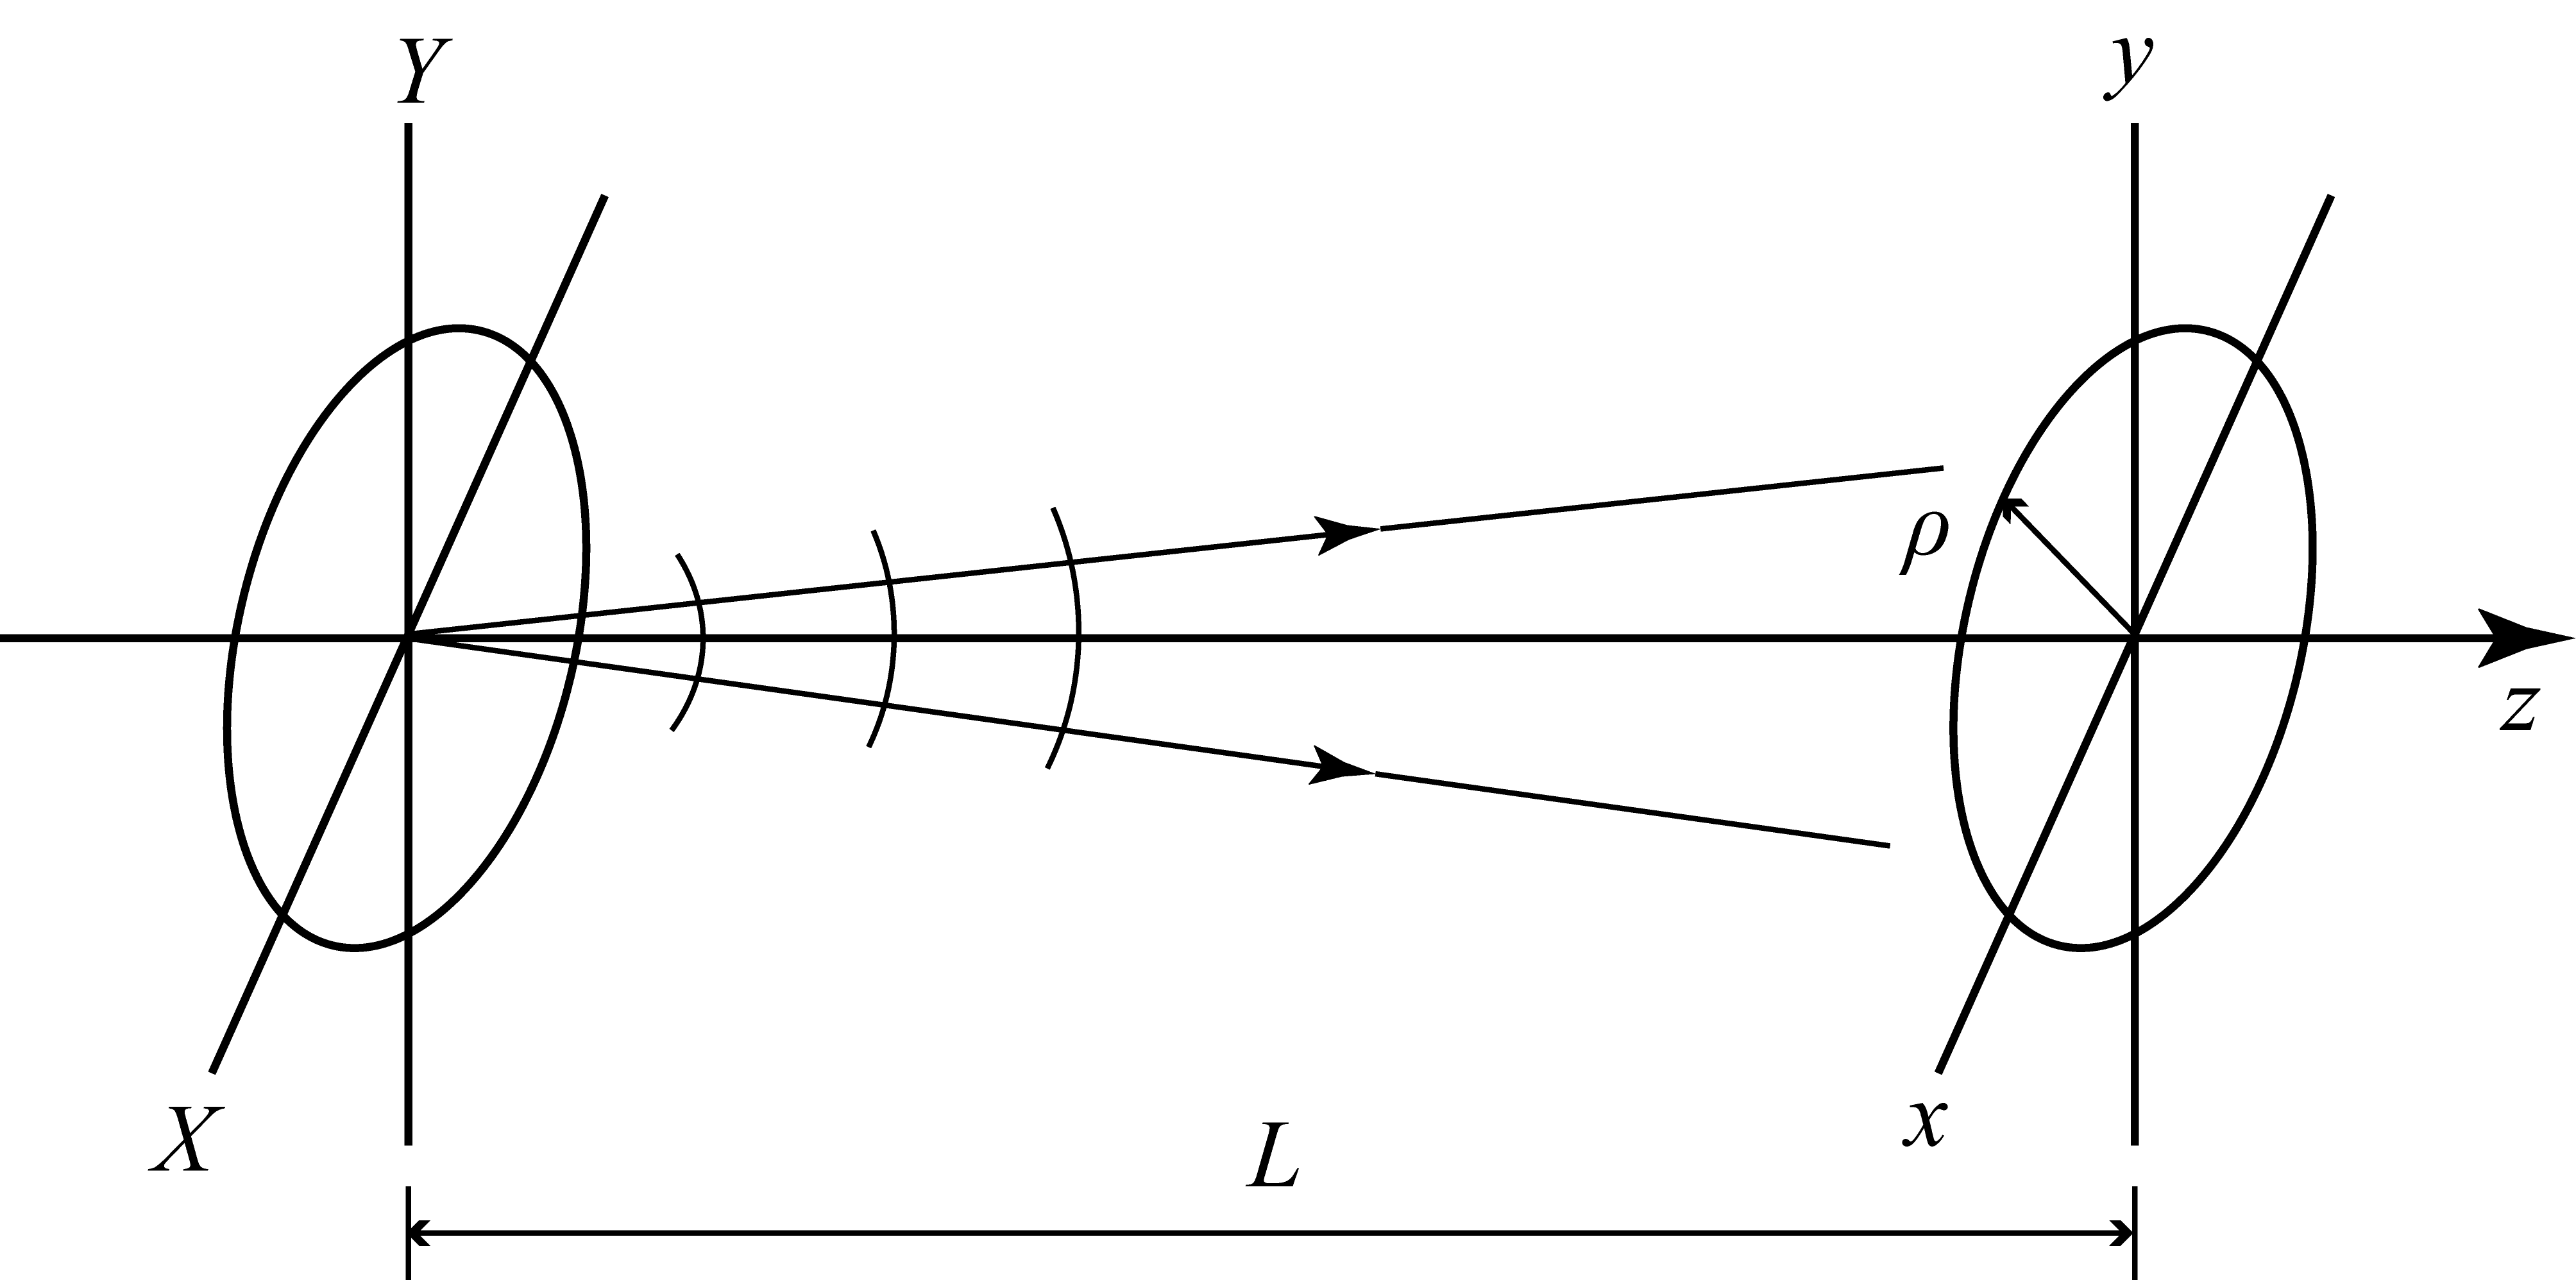
\includegraphics[width=10cm]{image/14-1-2.png}
\caption{球面波向平面波近似}
\end{wrapfigure}
但是旁边的点$(x_1,\,y_1)$的最佳平面波的近似却不一定平行于$z$轴,\,它应该为:
\[A(\bs{r})=A\ue^{\ui [k_z z+k_x (x-x_1)+k_y (y-y_1)]}\]

这下便有第一个近似条件了,\,我们叫做\emph{傍轴条件}(paraxial condition).\,它要求光线传播方向与$z$轴夹一个小角度.\,此时我们习惯把$x$和$y$方向方向余弦$\cos \alpha_x,\,\cos\alpha_y$使用的约$90$度的角度$\alpha_x,\,\alpha_y$的余角记做方向角,\,也就是说:
\[\sin \theta_x\approx \theta_x=\frac{k_x}{k}\quad,\quad \sin \theta_y\approx \theta_y=\frac{k_y}{k}\quad,\quad k_z\approx \sqrt{1-\theta^2_x-\theta^2_y}k\approx k\]

在傍轴近似下,\,以上以方向角$(\theta_x,\,\theta_y)$传播的平面波被方便地写为:
\[A(\bs{r})=A\ue^{\ui k z}\ue^{\ui\phi}\ue^{\ui k (\theta_x x+\theta_y y)}=A'\ue^{\ui k (\theta_x x+\theta_y y)}\]

经常的,\,我们只需要关心在像屏$z=0$上的场,\,参考上图.\,所以上式我们可以把不变的系数都统一写作$A'$.

但是平面波却不总是好的近似,\,我们已经发现了,\,像上图那样,\,如果在物屏$z=-L$上原点$X=0,\,Y=0$处有一点光源发出球面波,\,那么光屏上$(0,\,0)$处和$(x_1,\,y_1)$处的近似公式就采取了不同的形式.\,所以我们会寻求更好的球面波近似.\,但且慢,\,是不是任意情况下光场中的任意一点附近的场都能近似为一个球面波呢?\,答案显然是否定的.\,比如柱面波很显然就不能被近似为球面波,\,因为其\emph{波前}(wavefront),\,即等相位面沿垂直于传播方向的一个方向弯曲而另一个方向却是平直的.\,事实上球面波的光源是点,\,柱面波的光源是线.\,而介于柱面波与球面波中间的某种不对称波前就连光源都没法找到.\,但是球面波的地位仍然是重要的.\,这体现在两点上.\,一是在真实的光路系统中,\,点光源是切实存在且常用的.\,此时物方到像方的点到点的消除了像差的理想成像是我们努力追求的方向.\,故在这样的系统中光波的确一直都适合被近似为球面波,\,而平面波也被当做一种光源在无穷远的特殊状态而处理.\,二是,\,若把波前上各个点当成是新的次波源向前发射出球面波而在前方相干叠加形成新的光场,\,后面在衍射这一章我们数学上可以证明这就是计算光的传播的正确方式.\,其中用到的球面波作为一种本质上重要的物理对象,\,即\emph{传播子}(propagator),\,有着重要的物理地位.

故我们研究从物屏$z=-L$的$(X,\,Y)$处传播到像屏$z=0$处$(x,\,y)$点的球面波的场:
\begin{align*}
A(x,\,y)	&=\frac{I}{\sqrt{L^2+(x-X)^2+(y-Y)^2}}\ue^{\ui k\sqrt{L^2+(x-X)^2+(y-Y)^2}}\\
			&=\frac{I}{L}\ue^{\ui kL}\left[1+\frac{(x-X)^2}{L^2}+\frac{(y-Y)^2}{L^2}\right]^{-\frac{1}{2}}\ue^{\ui kL\left[\left[1+\frac{(x-X)^2}{L^2}+\frac{(y-Y)^2}{L^2}\right]^{\frac{1}{2}}-1\right]}
\end{align*}

由于傍轴条件,\,我们发现方向角$(u_x,\,u_y),\,u_x=\dfrac{x}{L},\,u_y=\dfrac{y}{L}$和方向角$(U_x,\,U_y),\,U_x=\dfrac{X}{L},\,U_y=\dfrac{Y}{L}$都是小量,\,而传播到光屏上该点的光的方向角($\bs{k}$方向)为$(u_x-U_x,\,u_y-U_y)$.\,仅考虑领头项,\,把不随$x,\,y$变化的系数记为常数,\,我们发现:
\[A(x,\,y)=A\ue^{\frac{\ui}{2}kL[(u_x-U_x)^2+(u_y-U_y)^2]}=A'\ue^{\ui k\frac{x^2+y^2}{2L}}\ue^{-\ui k\frac{Xx+Yy}{L}}\]

也就是说光屏上的波由两个相因子决定.\,第一个是平方相关于$x,\,y$的$\varphi_1=k\dfrac{x^2+y^2}{2L}=\pi \dfrac{x^2+y^2}{\lambda L}$,\,第二个恰好是平面波的相因子$\varphi_2=-k\dfrac{Xx+Yy}{L}=-k(U_x x+U_y y)=k(\theta_x x+\theta_y y)$.\,就是说当点光源相对$(x,\,y)=(0,\,0)$从$X<0,\,Y<0$的方向照过来能够在原点附近获得方向角为正的平面波场.

那么球面波能够被近似为球面波的条件也就不言自明了,\,它要求第一个相因子的相位很小不干扰第二个相因子,\,也就是$\varphi_1\ll \pi$,\,也就是\emph{远场条件}(farfield condition):
\[\rho^2\ll \lambda L\quad \Leftrightarrow \quad L\gg \frac{\rho^2}{\lambda}\]

其实换一个角度理解这个条件,\,如果远场条件被满足,\,但是在这样的$\rho$内第二个相因子变化也非常小时,\,整个$A$几乎就是常数,\,这时候也形成不了有价值的光场,\,所以我们如果要求$\varphi_2\gg \varphi_1$,\,还能发现第三个条件$X,\,Y\gg x,\,y$.\,对于这个条件我们做这样的理解,\,相位的绝对大小是没有观测效果的.\,我们需要的其实是光束干涉时相位的差值.\,故这其实是要求物屏的花样尺寸要远大于像屏上干涉花样的观测范围.

在远场条件不被满足的情况下,\,考虑第一个相因子对第二个相因子的影响,\,会造成干涉图样的扭曲与形变,\,几何光学上会造成最基础的像差:\,相散和散焦.

在介绍下两节具体的干涉之前,\,对干涉的原理做一个简要的介绍是有必要的.\,根据之前的介绍,\,空间中如果同时存在两个光场:
\[A_1(\bs{r})=|A_1|(\bs{r})\ue^{\ui\varphi_1(\bs{r})}\quad ;\quad A_2(\bs{r})=|A_2|(\bs{r})\ue^{\ui\varphi_2(\bs{r})}\]

我们可以找到其单独存在时的光强,\,一般来说,\,光强为位置的缓变函数:
\[I_1(\bs{r})=|A_1|^2=A_1^\ast A_1 \quad ;\quad I_2(\bs{r})=|A_2|^2=A_2^\ast A_2\]

然而光场的叠加是有两种典型的方式的.\,最常见的其实是\emph{非相干叠加}(incoherent superposition).\,此时出于下面要介绍的原因,\,光强是可以逐点直接相加的:
\[I(\bs{r})=I_1(\bs{r})+I_2(\bs{r})\]

将自然界或人造的两束来源不同的光照在一次是无法观察到干涉花样的.\,光的干涉条件比机械波干涉条件来的苛刻的多.\,在某些细心制备的实验室条件下才能观察到干涉花样,\,此时光场是\emph{相干叠加}(coherent superposition).\,在光学之中相干度是十分值得关注的.\,我们将在之后的一节中集中讨论.\,读者可能自然地认为相干叠加时为复振幅相加:
\[A(\bs{r})=A_1(\bs{r})+A_2(\bs{r})\]

但是其实无论非相干叠加还是相干叠加上式都适用,\,那么是什么造成了两者的区别呢?\,我们把上式模方求光强:
\begin{align*}
I(\bs{r}) &=A^\ast A \\
		  &=(A_1^\ast +A_2^\ast)(A_1+A_2) \\
		  &=A_1^\ast A_1+A_2^\ast A_2+ A_1^\ast A_2+A_2^\ast A_1 \\
		  &=I_1+I_2+ |A_1||A_2|\ue^{\ui (\varphi_2-\varphi_1)}+|A_1||A_2|\ue^{\ui (\varphi_1-\varphi_2)} \\
		  &=I_1+I_2+ 2\sqrt{I_1I_2}\cos (\varphi_2-\varphi_1)
\end{align*}

上式中出现的交叉项$2\sqrt{I_1I_2}\cos (\varphi_2-\varphi_1)$就叫\emph{干涉项}(interference term).\,它是关于位置的快变函数.\,乍一看这也未免太快了,\,因为只要当空间位置改变一个波长,\,相位$\varphi$就会有$\pi$的量级的改变,\,这样干涉项在这个过程中就会有正负号的改变.\,从而产生干涉花样.\,在实际的干涉实验中,\,合理的仪器设置可以使得这个空间特征长度被放大到人眼或助视仪器可以直接观测的程度.\,从而这就是干涉实验的基础.

那么为什么对于非相干叠加情形我们直接去掉了干涉项.\,那是因为在之前我们做把光场向标量复振幅简化的过程中去掉了公共的单色光时间演化项$\ue ^{\ui \omega t}$.\,这并不是永远合理的做法.\,真实光场由于后面要介绍的各种原因,\,可以认为相位随时间的演化并不是完全线性增加的而是有随时间偏离期望值的方差越来越大的涨落.\,从而两束并没有关联的自然光之间不同时刻同一点$\bs{r}$的相位差$\delta=\varphi_2(\bs{r})-\varphi_1(\bs{r})$是一个在随机涨落的数,\,只要涨落够大,\,$\cos (\varphi_2-\varphi_1)$项的随时间平均就会总是趋近于零.\,从而干涉现象也就消失了.

在以下的两小节中,\,我们先不用关心相干性的问题,\,认为不同光场的叠加总是有``完美的相干性'':\,完全稳定的相位差.\,我们会在不同干涉装置的介绍中去强调为什么总是能保证``完美的相干性''的成立.




\section{分波面干涉}

以下几种干涉装置一般统一归为\emph{分波面干涉}(interference by dividing wave-front).\,因为它们实现的核心思想都是让本来沿各个方向独立传播的波前的部分改变传播方式而在空间中产生交叠.

\subsection{杨氏双缝干涉仪}

历史上第一个挑战牛顿光的粒子说权威,\,构想出更合理的光的波动说的假设并通过实验证明自己的想法的是谁?\,那必然要归功于\emph{托马斯·杨}(Thomas Young)\footnote{杨氏为英国博物学家,\,也经常作为物理学家而介绍.\,除了双缝实验,\,也因为杨氏模量,\,杨-亥姆霍兹三色视觉论,\,杨-拉普拉斯和杨-杜普蕾附加压强与接触角公式而闻名.\,他还是杰出的语言学家,\,比较了400钟语言的词汇与语法.\,并解密了一部分古埃及象形文字.\,在音乐,\,医学和神学等上也有贡献.}.\,

\section{分振幅干涉}

\section{偏振干涉}

\section{相干性}

\section{多光束干涉}

